\documentclass[sigconf]{acmart}

% -----------------------------------------------------------------------
% Packages
% -----------------------------------------------------------------------
\usepackage{booktabs}
\usepackage{listings}
\usepackage{xcolor}
\usepackage{microtype}
\usepackage{graphicx}
\usepackage{amsmath}
\usepackage{tikz}
\usetikzlibrary{automata,positioning,arrows.meta}

% -----------------------------------------------------------------------
% Listing style for Aegis DSL
% -----------------------------------------------------------------------
\definecolor{aegisblue}{rgb}{0.13,0.37,0.68}
\definecolor{aegisgreen}{rgb}{0.16,0.52,0.20}
\definecolor{aegisgray}{rgb}{0.45,0.45,0.45}
\definecolor{aegispurple}{rgb}{0.50,0.10,0.55}

\lstdefinelanguage{Aegis}{
  morekeywords={policy, scope, on, rule, when, allow, deny, audit, redact,
                proof, invariant, always, eventually, never, until, before,
                after, next, within, rate_limit, quota, per, import, from,
                as, extends, let, def, type, match, true, false, all, any,
                none, exists, count, log, notify, escalate, block, tag,
                critical, high, medium, low, info, and, or, not, in,
                implies},
  sensitive=true,
  morecomment=[l]{//},
  morecomment=[s]{/*}{*/},
  morestring=[b]",
  keywordstyle=\color{aegisblue}\bfseries,
  commentstyle=\color{aegisgray}\itshape,
  stringstyle=\color{aegisgreen},
  basicstyle=\ttfamily\small,
  numbers=left,
  numberstyle=\tiny\color{aegisgray},
  frame=single,
  breaklines=true,
  captionpos=b
}

\lstset{language=Aegis}

% -----------------------------------------------------------------------
% Metadata
% -----------------------------------------------------------------------
\title{AutomaGuard: Compiled Temporal Policy Enforcement for Production AI Agents}

\author{Scott Davis}
\affiliation{%
  \institution{Independent}
  \city{[City]}
  \country{[Country]}
}
\email{[author@email]}

\begin{abstract}
AI agents that invoke external tools, access sensitive data, and operate with
minimal human supervision require safety guarantees stronger than best-effort
guardrails. We present \textbf{AutomaGuard}, a formal policy enforcement engine
that provides mathematical guarantees---not probabilistic estimates---that
agent behavior complies with specified constraints. AutomaGuard comprises three
components: (1)~the \textbf{Aegis Policy Language}, a domain-specific language
in which policies are expressed as typed rules and temporal invariants;
(2)~an \textbf{ahead-of-time compiler} that translates Aegis source to
deterministic state machines encoded in a compact bytecode format; and
(3)~a \textbf{Rust runtime verifier} that intercepts agent events, evaluates
compiled rules, advances automaton state, and enforces sliding-window rate
limits---all within a sub-10\,ms per-event latency budget.

Unlike static workflow analyzers, AutomaGuard evaluates the \emph{actual}
execution trace of a running agent, catching violations that only manifest
from runtime data (e.g., PII in an LLM response, a specific tool-call sequence
not predictable from the graph topology). Unlike runtime guardrails that
interpret policy at request time, AutomaGuard compiles policies to state machines
ahead of deployment, eliminating parsing overhead and enabling a hard latency
guarantee. Benchmarks on a realistic policy (10 rules, 2 state machines, 1 rate
limiter) show a mean evaluation latency of 2.4\,\textmu s---more than 4$\times$
within the 10\,ms budget---with throughput exceeding 1.3 million events per
second. A Python SDK with LangChain and OpenAI integrations enables drop-in
enforcement with three lines of user code.
\end{abstract}

\keywords{AI agents, policy enforcement, formal verification, temporal logic,
runtime monitoring, domain-specific language, Rust, safety}

\sloppy  % allow loose line-breaking to prevent overfull hboxes in two-column

\begin{document}
\maketitle

% -----------------------------------------------------------------------
\section{Introduction}
% -----------------------------------------------------------------------

The deployment of AI agents in production settings introduces a qualitatively
different risk profile from traditional software. Where a conventional
application executes a deterministic program, an agent driven by a large
language model (LLM) operates by selecting and invoking tools dynamically in
response to inputs whose distribution is open-ended. A single agent session may
traverse tool-call sequences that were never tested, involving sensitive
resources such as customer PII, financial accounts, or privileged
infrastructure APIs.

Existing approaches to constraining agent behavior fall into two categories,
each with fundamental limitations:

\paragraph{Runtime guardrails (interpreted).}
Tools such as NeMo Guardrails~\cite{rebedea2023nemo}, LlamaGuard~\cite{inan2023llama},
and Guardrails AI intercept individual outputs and evaluate them against rules
expressed as prompts, classifiers, or regular expressions. These tools operate
on a per-call basis: they cannot reason about \emph{sequences} of events or
enforce invariants that span multiple turns. Moreover, they re-parse or
re-run inference at every evaluation, introducing latency that scales with
policy complexity and model size.

\paragraph{Static workflow analyzers.}
Recent work~\cite{xavier2026agentproof} extracts graph models from agent
frameworks and applies pre-deployment checks against temporal safety policies
compiled to deterministic finite automata. Static analysis provides
path-exhaustive guarantees but is fundamentally limited to properties derivable
from the graph topology. It cannot catch violations conditioned on runtime
values---for example, that the \emph{content} of a specific API response
triggers a forbidden downstream action---and offers no enforcement mechanism
during live execution.

AutomaGuard occupies a third position: \textbf{compiled runtime enforcement}.
Policies are expressed in a typed DSL with first-class temporal operators,
compiled ahead of deployment to state machines, and evaluated against the live
event stream at sub-microsecond latency per event. This design provides:

\begin{enumerate}
  \item \textbf{Sequence-level guarantees.} Temporal invariants expressed with
    \texttt{always}, \texttt{eventually}, \texttt{never}, and \texttt{until}
    compile to automata that detect violations spanning arbitrary-length event
    sequences---the moat that per-call guardrails cannot cross.
  \item \textbf{Hard latency bounds.} Because there is no policy parsing at
    evaluation time, the latency is determined entirely by rule evaluation and
    state-machine stepping---operations that are $O(\text{rules} + \text{automata})$
    in the compiled policy, not $O(\text{policy source size})$.
  \item \textbf{Runtime data sensitivity.} Policies can condition on event field
    values, PII markers, tool argument contents, and aggregated statistics, all
    of which are only known at runtime.
  \item \textbf{Append-only audit trail.} Every verdict, with its triggering
    event, matched rules, automaton transitions, and evaluation latency, is
    logged immutably.
\end{enumerate}

This paper makes the following contributions:
\begin{itemize}
  \item The design and implementation of the \textbf{Aegis Policy Language}:
    syntax, type system with subtyping, temporal operators, rate-limit
    declarations, and policy inheritance (\S\ref{sec:aegis}).
  \item A \textbf{compilation pipeline} from Aegis source to verified IR and
    compact \texttt{.aegisc} bytecode, including the state-machine construction
    algorithm for temporal invariants (\S\ref{sec:compiler}).
  \item A \textbf{Rust runtime verifier} with allocation-minimal evaluation,
    sliding-window rate limiters, and an append-only ring-buffer audit log
    (\S\ref{sec:runtime}).
  \item A \textbf{Python SDK} providing drop-in enforcement for LangChain and
    OpenAI agents via pyo3 bindings (\S\ref{sec:sdk}).
  \item \textbf{Evaluation} demonstrating sub-10\,ms p99 latency with 4$\times$
    headroom on realistic policies (\S\ref{sec:eval}).
\end{itemize}


% -----------------------------------------------------------------------
\section{Motivation and Threat Model}
\label{sec:motivation}
% -----------------------------------------------------------------------

\subsection{Representative Agent Threats}

We motivate the design with two attack patterns that appear in the
\texttt{research\_guard.aegis} and \texttt{data\_exfiltration\_guard.aegis}
example policies included in the AutomaGuard distribution.

\paragraph{Indirect prompt injection via action sequences.}
An adversarial document instructs an agent to (a)~search for sensitive files,
then (b)~email their contents to an external address. Each action in isolation
may be permitted by per-call rules---searching and emailing are both legitimate
capabilities. Only the \emph{sequence} ``file access of sensitive material
followed by email to external recipient'' is the violation. A per-call guardrail
cannot detect this pattern; a temporal invariant over the event stream can.

\paragraph{PII exfiltration via tool arguments.}
An agent processing customer records may inadvertently include PII in
the arguments to a third-party tool call. The violation is conditioned on the
\emph{content} of a specific runtime field, not on the workflow topology.
Static analysis cannot detect it; a runtime rule that inspects tool-call
arguments can.

\subsection{Threat Model}

AutomaGuard targets the following threats:

\begin{description}
  \item[T1 Developer mistakes.] Agent developers write policies that compile
    successfully but contain logical gaps (e.g., missing human-gate on a
    sensitive path). The compiler's type checker and diagnostic system surface
    these at compile time.
  \item[T2 Adversarial sequences.] An adversary (via prompt injection or
    tool-call manipulation) orchestrates a sequence of actions that individually
    pass per-call checks but collectively violate a policy. Temporal invariants
    catch these.
  \item[T3 Rate-based abuse.] An agent is induced to call an external API or
    read sensitive data at a rate that reveals information or causes cost
    overruns. Sliding-window rate limiters enforce budgets.
  \item[T4 Runtime data violations.] A policy condition depends on the
    \emph{value} of a field known only at runtime (PII marker, classification
    level, response content). Runtime expression evaluation catches these.
\end{description}

\noindent AutomaGuard does not address semantic correctness of LLM outputs
(factuality, intent), non-deterministic agent topology, or threats arising from
the model weights themselves.


% -----------------------------------------------------------------------
\section{The Aegis Policy Language}
\label{sec:aegis}
% -----------------------------------------------------------------------

Aegis is a statically typed, declarative DSL for expressing agent behavioral
constraints. A policy is a named collection of rules, constraints, proofs, and
(optionally) type and function definitions. Policies may extend a base policy,
inheriting its rules and adding or overriding members.

\subsection{Syntax Overview}

Listing~\ref{lst:simple} shows a minimal policy demonstrating the core
language elements.

\begin{lstlisting}[caption={A minimal Aegis policy.},label={lst:simple}]
policy DataGuard {
  // Rate limit: max 100 tool calls per minute
  rate_limit tool_calls: 100 per 1m

  // Per-event rule
  on tool_call {
    when event.tool_name == "drop_table"
    deny "DDL operations are prohibited"
    severity critical
  }

  on external_request {
    when !is_approved(event.endpoint)
    audit "Unapproved endpoint"
    severity high
  }

  // Temporal invariant: PII never reaches a tool call
  proof PIIContainment {
    invariant NoPIIInArgs {
      never(any(event.arguments, arg =>
        arg.classification == "PII"))
    }
  }
}
\end{lstlisting}

\subsection{Event Model}

Every agent action is represented as an \emph{event}: a typed pair
$(\textit{event\_type}, \textit{fields})$ where \textit{fields} is a string-keyed
map of runtime-typed values. The built-in event types and their field schemas are:

\begin{center}
\begin{tabular}{ll}
\toprule
Event type & Key fields \\
\midrule
\texttt{tool\_call} & \texttt{tool\_name}, \texttt{arguments}, \texttt{result} \\
\texttt{external\_request} & \texttt{endpoint}, \texttt{method}, \texttt{body} \\
\texttt{data\_access} & \texttt{resource}, \texttt{classification} \\
\texttt{message} & \texttt{role}, \texttt{content} \\
\texttt{file\_access} & \texttt{path}, \texttt{operation} \\
\texttt{code\_execution} & \texttt{language}, \texttt{code} \\
\bottomrule
\end{tabular}
\end{center}

\subsection{Type System}

Aegis has a structural type system with subtyping. The primitive types are
\texttt{int}, \texttt{float}, \texttt{bool}, \texttt{string}, and
\texttt{duration} (e.g., \texttt{5ms}, \texttt{10s}, \texttt{24h}).
Collection types include \texttt{List<T>}, \texttt{Map<K,V>}, and
\texttt{Set<T>}. Union types (\texttt{A | B}) are supported. User-defined
struct types are declared with \texttt{type}.

Subtyping rules are:
\begin{itemize}
  \item \texttt{never} is the bottom type (subtype of all types).
  \item \texttt{int} $\sqsubseteq$ \texttt{float} (numeric widening).
  \item $T \sqsubseteq T \mid U$ and $U \sqsubseteq T \mid U$ (union
    introduction).
  \item Collections are covariant: \texttt{List<int>} $\sqsubseteq$
    \texttt{List<float>}.
\end{itemize}

\subsection{Rule Clauses}

A rule is triggered when an event matches its \texttt{on} declaration.
The body consists of:
\begin{itemize}
  \item Zero or one \texttt{when} clause (a boolean expression; omitting it
    means the rule fires on every matching event).
  \item One or more verdict clauses: \texttt{allow}, \texttt{deny},
    \texttt{audit} (log but allow), or \texttt{redact} (allow but sanitize
    output).
  \item Optional action clauses: \texttt{log}, \texttt{notify},
    \texttt{escalate}, \texttt{block}, \texttt{tag}.
  \item An optional severity annotation: \texttt{critical}, \texttt{high},
    \texttt{medium}, \texttt{low}, \texttt{info}.
\end{itemize}

When multiple rules fire on a single event, \texttt{deny} takes precedence over
all other verdicts; among equal-precedence verdicts the first-fired rule wins.

\subsection{Temporal Operators}
\label{sec:temporal}

Temporal invariants are placed inside \texttt{proof} blocks. The language
supports the following operators, corresponding to the stated LTL formulae over
the event stream $\sigma = e_0, e_1, e_2, \ldots$:

\begin{center}
\begin{tabular}{lll}
\toprule
Aegis syntax & LTL formula & Intuition \\
\midrule
\texttt{always($\phi$)} & $\square\phi$ & $\phi$ holds on every event \\
\texttt{never($\phi$)} & $\square\neg\phi$ & $\phi$ never holds \\
\texttt{eventually($\phi$) within T} & $\lozenge_{\leq T}\phi$ & $\phi$ holds within deadline $T$ \\
\texttt{until($\phi$, $\psi$)} & $\phi \,\mathcal{U}\, \psi$ & $\phi$ holds until $\psi$ \\
\texttt{before($\phi$, $\psi$)} & $\phi \,\mathcal{U}\, \psi$ & $\phi$ precedes $\psi$ \\
\texttt{after($\phi$, $\psi$)} & $\psi \Rightarrow \lozenge\phi$ & after $\psi$, $\phi$ must follow \\
\texttt{next($\phi$)} & $\mathcal{X}\phi$ & $\phi$ holds on the next event \\
\bottomrule
\end{tabular}
\end{center}

\noindent The expressions $\phi$ and $\psi$ are full Aegis boolean expressions
over the current event's fields, supporting quantifiers (\texttt{all},
\texttt{any}, \texttt{none}, \texttt{exists}), string predicates
(\texttt{contains}, \texttt{matches}, \texttt{starts\_with}), arithmetic, and
user-defined functions.

\paragraph{Composing temporal and data predicates.}
Aegis's key expressive advantage over approaches that restrict to fixed property
templates is the ability to compose temporal operators with arbitrary data
predicates. For example, the following invariant detects the indirect-injection
attack from \S\ref{sec:motivation}:

\begin{lstlisting}[caption={Sequence-level exfiltration detection.},label={lst:seq}]
proof ExfiltrationDetection {
  invariant NoPIIFollowedByExternalSend {
    never(
      after(
        event.event_type == "external_request"
          && event.endpoint matches r".*@.*",
        event.event_type == "data_access"
          && event.classification == "PII"
      )
    )
  }
}
\end{lstlisting}

\subsection{Rate Limits and Quotas}

Rate limits are declared at policy scope:

\begin{lstlisting}[numbers=none]
rate_limit tool_calls:         100 per 1m
rate_limit external_requests:  20  per 5m
quota      data_reads:         10000 per 1h
\end{lstlisting}

\noindent The runtime enforces these with sliding-window counters
(\S\ref{sec:ratelimit}), which prevents burst-at-window-boundary exploits that
fixed-window counters are susceptible to.

\subsection{Policy Inheritance}

A policy may extend exactly one base policy using the \texttt{extends} keyword.
Inheritance is single (no diamonds). The derived policy inherits all rules,
constraints, and proof blocks from the base and may add new members or override
specific rules by name. This enables a common pattern of a strict production
policy with a more permissive development variant:

\begin{lstlisting}[numbers=none]
policy DevMode extends DataGuard {
  on tool_call {
    when event.environment == "development"
    allow
  }
}
\end{lstlisting}


% -----------------------------------------------------------------------
\section{Compilation Pipeline}
\label{sec:compiler}
% -----------------------------------------------------------------------

Figure~\ref{fig:pipeline} shows the five-stage compilation pipeline from
Aegis source to \texttt{.aegisc} bytecode.

\begin{figure}[t]
\centering
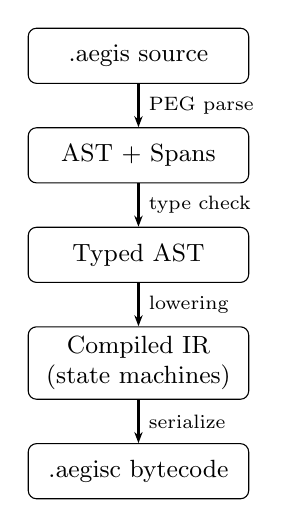
\begin{tikzpicture}[
  node distance=0.55cm,
  box/.style={draw, rounded corners=3pt, minimum width=2.8cm,
              minimum height=0.7cm, font=\small, align=center},
  arrow/.style={-{Stealth[length=4pt]}, thick}
]
\node[box] (src)  {.aegis source};
\node[box, below=of src] (ast)  {AST + Spans};
\node[box, below=of ast] (tast) {Typed AST};
\node[box, below=of tast] (ir)  {Compiled IR\\(state machines)};
\node[box, below=of ir]  (bc)   {.aegisc bytecode};

\draw[arrow] (src)  -- node[right,font=\scriptsize]{PEG parse} (ast);
\draw[arrow] (ast)  -- node[right,font=\scriptsize]{type check} (tast);
\draw[arrow] (tast) -- node[right,font=\scriptsize]{lowering} (ir);
\draw[arrow] (ir)   -- node[right,font=\scriptsize]{serialize} (bc);
\end{tikzpicture}
\caption{Aegis compilation pipeline.}
\Description{Flow diagram showing five compilation stages: .aegis source to AST with Spans (PEG parse), to Typed AST (type check), to Compiled IR with state machines (lowering), to .aegisc bytecode (serialize).}
\label{fig:pipeline}
\end{figure}

\subsection{Parsing}

The parser is generated from a PEG grammar using the \texttt{pest} crate.
The grammar is organized into three layers:
\begin{enumerate}
  \item \textbf{Lexical}: keywords, identifiers, literals (bool, int, float,
    duration, string, raw string \texttt{r"..."}, regex \texttt{r/\ldots/}).
  \item \textbf{Expressions}: full expression grammar with precedence climbing
    (binary operators, unary, predicates, quantifiers, lambdas, \texttt{match}
    expressions, temporal sub-expressions).
  \item \textbf{Declarations}: \texttt{policy}, \texttt{proof}, \texttt{type},
    \texttt{let}, \texttt{def}, \texttt{import}, with annotation support
    (\texttt{@name(args)}).
\end{enumerate}

Every AST node carries a \texttt{Spanned<T>} wrapper recording its byte range
in the source file. All diagnostic messages produced by later passes include
source spans, enabling IDE-quality error reporting.

\subsection{Type Checking}

The type checker runs in two passes to support forward references:

\begin{enumerate}
  \item \textbf{Registration pass}: Collect all top-level type and function
    declarations into the type environment.
  \item \textbf{Body pass}: Recursively check all expression bodies, rule
    clauses, and proof blocks.
\end{enumerate}

A \texttt{CheckContext} tracks whether the checker is currently inside a
\texttt{proof}/\texttt{invariant} block (where temporal operators are
permitted), a \texttt{rule} body, and the current temporal nesting depth (v1
limits to depth 1 to keep automaton construction tractable). The type checker
enforces structural invariants including: temporal operators only in proof
contexts; \texttt{when} clauses must be boolean; rate-limit windows must be
\texttt{duration} typed; function argument counts match declarations.

The checker emits diagnostics into a \texttt{DiagnosticSink} rather than
aborting on the first error, allowing all errors in a policy file to be
reported in a single compilation pass (comparable to the Rust compiler's
``multiple error'' reporting model).

\subsection{Lowering and State-Machine Construction}
\label{sec:lowering}

The lowering pass transforms the typed AST into \texttt{CompiledPolicy}, the
IR that is serialized to \texttt{.aegisc} bytecode and consumed by the runtime.

\paragraph{Inheritance resolution.}
The lowering pass builds a policy inheritance map and resolves the
\texttt{extends} chain for each policy (single-inheritance, so $O(d)$ where
$d$ is the inheritance depth). Inherited members are collected base-first.

\paragraph{Expression lowering.}
AST expressions are lowered to \texttt{IRExpr}, a type-erased,
allocation-minimal representation suitable for tight evaluation loops. Variable
references are resolved to slot indices (\texttt{RefRoot::Local(n)}). Match
expressions are compiled to \texttt{DecisionTree} nodes for efficient dispatch.

\paragraph{Temporal to state machine.}
Each temporal invariant in a \texttt{proof} block is compiled to a
\texttt{StateMachine} value. The construction depends on the outermost temporal
operator:

\begin{description}
  \item[\texttt{always($\phi$)}] Two-state machine: initial state $s_0$
    (active/satisfied); transition to $s_1$ (violated, absorbing) on
    $\neg\phi$.
  \item[\texttt{never($\phi$)}] Two-state machine: initial state $s_0$
    (active/satisfied); transition to $s_1$ (violated, absorbing) on $\phi$.
  \item[\texttt{eventually($\phi$) within T}] Three-state machine: $s_0$
    (waiting); transition to $s_1$ (satisfied, absorbing) on $\phi$; transition
    to $s_2$ (violated, absorbing) on timeout $T$ if still in $s_0$.
  \item[\texttt{until($\phi$, $\psi$)}] Three-state machine: $s_0$ (holding);
    transition to $s_1$ (released, absorbing) on $\psi$; transition to $s_2$
    (violated, absorbing) on $\neg\phi \wedge \neg\psi$.
  \item[\texttt{after($\phi$, trigger)}] Three-state machine: $s_0$ (waiting
    for trigger); transition to $s_1$ (triggered, monitoring) on \textit{trigger};
    from $s_1$, transition to $s_2$ (satisfied, absorbing) on $\phi$, remain in
    $s_1$ if not yet $\phi$.
\end{description}

Figure~\ref{fig:automata} illustrates the \texttt{always} and
\texttt{eventually within T} automata.

\begin{figure}[t]
\centering
% --- always automaton ---
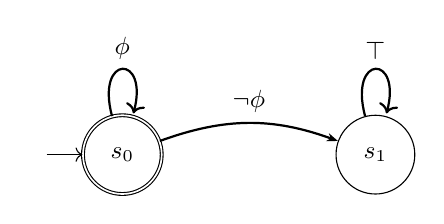
\begin{tikzpicture}[
  every state/.style={draw, circle, minimum size=1.0cm, font=\small},
  accepting/.style={double},
  arrow/.style={-{Stealth[length=4pt]}, thick},
  node distance=2.2cm
]
\node[state, accepting, initial, initial text={}] (s0) {$s_0$};
\node[state, right=of s0] (s1) {$s_1$};
\draw[arrow] (s0) edge[bend left=20] node[above]{\small $\neg\phi$} (s1);
\draw[arrow] (s0) edge[loop above] node[above]{\small $\phi$} ();
\draw[arrow] (s1) edge[loop above] node[above]{\small $\top$} ();
\end{tikzpicture}

\bigskip
% --- eventually within T automaton ---
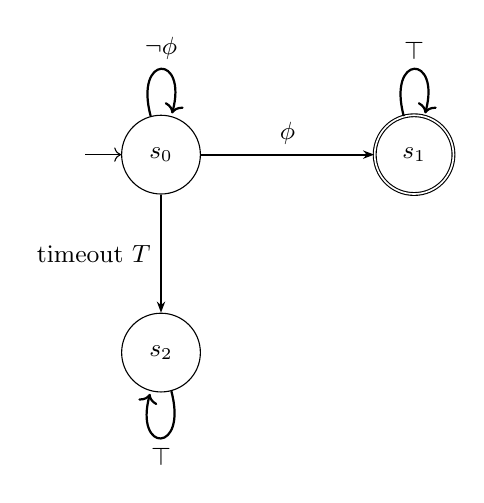
\begin{tikzpicture}[
  every state/.style={draw, circle, minimum size=1.0cm, font=\small},
  accepting/.style={double},
  arrow/.style={-{Stealth[length=4pt]}, thick},
  node distance=2.2cm
]
\node[state, initial, initial text={}] (w) {$s_0$};
\node[state, accepting, right=of w] (s) {$s_1$};
\node[state, below=1.5cm of w] (v) {$s_2$};
\draw[arrow] (w) edge node[above]{\small $\phi$} (s);
\draw[arrow] (w) edge[loop above] node[above]{\small $\neg\phi$} ();
\draw[arrow] (w) edge node[left]{\small timeout $T$} (v);
\draw[arrow] (s) edge[loop above] node[above]{\small $\top$} ();
\draw[arrow] (v) edge[loop below] node[below]{\small $\top$} ();
\end{tikzpicture}

\caption{State machines for \texttt{always}($\phi$) (top) and
\texttt{eventually}($\phi$) \texttt{within T} (bottom). $s_0$: active;
$s_1$: satisfied (accepting); $s_2$: violated (absorbing). Double circles
denote accepting/non-violating states.}
\Description{Two automata diagrams. Top (always): two states s0 (accepting, initial) and s1 (violated); s0 self-loops on phi, transitions to s1 on not-phi; s1 self-loops on true. Bottom (eventually within T): three states s0 (initial), s1 (accepted), s2 (violated); s0 transitions to s1 on phi, self-loops on not-phi, transitions to s2 on timeout T; s1 and s2 self-loop on true.}
\label{fig:automata}
\end{figure}

\subsection{Bytecode Format}

The \texttt{.aegisc} format is a self-describing binary envelope:

\begin{center}
\begin{tabular}{llr}
\toprule
Field & Content & Size \\
\midrule
Magic & \texttt{0xAE915C01} & 4 bytes \\
Version & \texttt{0x0001} & 2 bytes \\
Flags & reserved & 2 bytes \\
Payload length & little-endian uint32 & 4 bytes \\
Payload & JSON-serialized \texttt{CompiledPolicy} & variable \\
\bottomrule
\end{tabular}
\end{center}

\noindent The magic number encodes a mnemonic (\texttt{AEGIS}) and the major
version in the low byte, enabling version detection without full deserialization.
The JSON payload format is human-inspectable via the \texttt{aegisc inspect}
subcommand, which aids policy debugging and audit.


% -----------------------------------------------------------------------
\section{Runtime Verifier}
\label{sec:runtime}
% -----------------------------------------------------------------------

\subsection{Event Evaluation}

The \texttt{PolicyEngine} owns a deserialized \texttt{CompiledPolicy}, a vector
of \texttt{StateMachineInstance} values, a map of \texttt{RateLimiter} values,
and a \texttt{context} map of persistent per-session state. It exposes a single
primary method:

\begin{center}
\texttt{evaluate(event: \&Event) -> PolicyResult}
\end{center}

The evaluation algorithm (\texttt{engine.rs}) runs in five steps:
\begin{enumerate}
  \item \textbf{Rate-limit check.} For each \texttt{CompiledConstraint},
    invoke the corresponding \texttt{RateLimiter::record}. If any limiter
    exceeds its budget, return \texttt{Verdict::Deny} immediately.
  \item \textbf{Rule evaluation.} Iterate compiled rules in order. For each
    rule, check event-type membership (O(1) SmolStr comparison). If the rule
    applies, evaluate the optional \texttt{when} condition using the expression
    evaluator. Collect verdicts and actions from matching rules.
  \item \textbf{Verdict resolution.} \texttt{Deny} overrides all others;
    among the remainder, \texttt{Audit} and \texttt{Redact} override
    \texttt{Allow}.
  \item \textbf{State-machine stepping.} For each \texttt{StateMachineInstance}
    not in a terminal state, call \texttt{step(eval\_ctx, now\_ms)}. Collect
    any transitions to violating states.
  \item \textbf{Result construction.} Assemble \texttt{PolicyResult} with
    verdict, reason, triggered rule IDs, actions, violations, and evaluation
    latency in microseconds.
\end{enumerate}

\subsection{Expression Evaluator}

The expression evaluator (\texttt{eval.rs}) recursively reduces \texttt{IRExpr}
trees against an \texttt{EvalContext} holding the current event, session context,
policy configuration, and local variable slots. Design goals are:

\begin{itemize}
  \item \textbf{Allocation-minimal.} The hot path avoids heap allocation
    for scalar results. Collections allocate only when constructed by the
    expression, not on every traversal.
  \item \textbf{Short-circuit.} \texttt{\&\&} and \texttt{||} short-circuit
    as in standard evaluation. The \texttt{implies} operator (\texttt{a implies
    b}) is equivalent to \texttt{!a || b} and short-circuits when \texttt{a}
    is false.
  \item \textbf{Numeric coercion.} Cross-type comparisons between
    \texttt{Int} and \texttt{Float} values coerce \texttt{Int} to \texttt{Float}
    without panicking, matching the type system's subtyping rule.
  \item \textbf{Quantifier streaming.} \texttt{all}, \texttt{any},
    \texttt{none}, and \texttt{exists} iterate their collection without
    materializing an intermediate result vector.
\end{itemize}

The runtime's \texttt{Value} type is a six-variant enum covering \texttt{Null},
\texttt{Bool}, \texttt{Int(i64)}, \texttt{Float(f64)},
\texttt{String(SmolStr)}, \texttt{Duration(u64)}, \texttt{List(Vec<Value>)},
and \texttt{Map(HashMap<SmolStr, Value>)}.

\subsection{State-Machine Execution}

Each \texttt{StateMachineInstance} wraps the compiled \texttt{StateMachine}
specification and tracks the current state ID and start timestamp.
\texttt{step(ctx, now\_ms)} evaluates transitions from the current state:
\begin{enumerate}
  \item If a \texttt{Timeout} guard is present and the elapsed time since
    \texttt{start\_time\_ms} exceeds \texttt{deadline\_millis}, fire the
    timeout transition.
  \item Otherwise, evaluate each predicate-guarded transition in order; fire
    the first whose guard evaluates to true.
\end{enumerate}

Violated and satisfied states are absorbing (self-loop with $\top$ guard), so
the step function returns immediately once a terminal state is reached. This
bounds per-event automaton work to $O(|\delta|)$ where $|\delta|$ is the number
of transitions from the current state (typically 1--3).

\subsection{Sliding-Window Rate Limiters}
\label{sec:ratelimit}

Each \texttt{CompiledConstraint} with \texttt{kind = RateLimit} or
\texttt{kind = Quota} is paired with a \texttt{RateLimiter} that maintains a
timestamp vector implementing a sliding window:

\begin{enumerate}
  \item Compute \texttt{window\_start = now\_ms - window\_millis}.
  \item Evict all entries $< \texttt{window\_start}$ from the front of the
    timestamp vector (amortized $O(1)$ per call).
  \item Append \texttt{now\_ms} to the vector.
  \item If \texttt{len() > limit}, return \texttt{exceeded}.
\end{enumerate}

The sliding-window design ensures that a burst of exactly \texttt{limit}
events at the boundary of two fixed windows (each window's count appearing
at half the limit) cannot bypass enforcement. The memory cost is $O(L)$ per
limiter where $L$ is the limit value.

\subsection{Audit Log}

The audit log is an append-only ring buffer of \texttt{AuditEntry} values,
each recording: policy name, event type, verdict, reason, triggered rules,
violations, evaluation latency, and a monotonic timestamp. The ring buffer
has a configurable maximum size; when full, the oldest entry is overwritten.
The \texttt{total\_recorded} counter is never decremented, enabling external
auditors to detect gaps.

Entries can be queried by verdict type, event type, violation presence, or
recency, and serialized to JSON for export to external SIEM systems. An
optional file-flush path writes entries synchronously to a local append-only
log file.

\subsection{Fail-Closed Semantics}

Any error in rule evaluation (type mismatch, missing field, division by zero)
returns \texttt{Value::Null}, which is falsy; conditions that evaluate to
\texttt{Null} are treated as unmatched. At the Python SDK layer, any exception
from the Rust engine results in a \texttt{deny} verdict with an error reason.
This fail-closed contract ensures that an unanticipated policy input cannot
silently bypass enforcement.


% -----------------------------------------------------------------------
\section{Python SDK}
\label{sec:sdk}
% -----------------------------------------------------------------------

AutomaGuard provides a Python SDK built on pyo3, enabling native-performance
policy enforcement within Python-based agent frameworks. The SDK design
principle is ``Python as skin, not brain'': all evaluation logic lives in
Rust; the Python layer is a thin adapter.

\subsection{Core API}

\begin{lstlisting}[language=Python,caption={Drop-in enforcement with three lines.},label={lst:sdk}]
from aegis_enforce import enforce

# Wrap any OpenAI or LangChain client
safe_client = enforce(client, policy="guard.aegisc")

# Use identically to the unwrapped client
response = safe_client.chat.completions.create(...)
\end{lstlisting}

The \texttt{enforce()} function returns a proxy object that intercepts tool
calls, evaluates them against the loaded policy, and either passes them through
or raises \texttt{EnforcementError} depending on the verdict. An \texttt{audit}
verdict passes through but records the event; a \texttt{redact} verdict
sanitizes the response before returning it to the caller.

\subsection{Framework Integrations}

\paragraph{OpenAI.}
The OpenAI integration wraps \texttt{openai.OpenAI} with a proxy that
intercepts \texttt{chat.completions.create} calls. Tool calls embedded in
assistant messages are extracted, evaluated as \texttt{tool\_call} events,
and blocked if denied.

\paragraph{LangChain.}
The LangChain integration provides an \texttt{AutomaGuardCallbackHandler}
implementing the \texttt{BaseCallbackHandler} interface. Hooks fire on
\texttt{on\_tool\_start}, \texttt{on\_tool\_end}, and \texttt{on\_tool\_error},
converting LangChain's callback arguments to AutomaGuard events and raising
\texttt{EnforcementError} on denial.

\subsection{Direct Engine Access}

For frameworks not yet natively integrated, the \texttt{PolicyEngine} class
is exposed directly:

\begin{lstlisting}[language=Python,caption={Direct engine access.},label={lst:engine}]
from aegis_enforce import PolicyEngine

engine = PolicyEngine.from_file("guard.aegisc")
result = engine.evaluate("tool_call", {
    "tool_name": "send_email",
    "arguments": {"to": "user@example.com",
                  "body": context["draft"]}
})
if result["verdict"] == "deny":
    raise RuntimeError(result["reason"])
\end{lstlisting}

The \texttt{evaluate()} method returns a plain Python dictionary, keeping the
API dependency-free for callers that do not use the framework-specific wrappers.


% -----------------------------------------------------------------------
\section{Evaluation}
\label{sec:eval}
% -----------------------------------------------------------------------

\subsection{Latency Benchmarks}

We evaluate runtime latency using Criterion.rs (a statistically rigorous
benchmarking library) on a Linux workstation. Table~\ref{tab:bench} reports
mean latency and headroom under the 10\,ms budget across seven policy
scenarios.

\begin{table}[t]
\centering
\caption{Per-event evaluation latency (Criterion.rs mean). $R$ = rules,
$S$ = state machines, $L$ = rate limiters.}
\label{tab:bench}
\begin{tabular}{lrrrl}
\toprule
Scenario & $R$ & $S$ & $L$ & Mean latency \\
\midrule
Baseline (empty policy) & 0 & 0 & 0 & 38\,ns \\
Single allow rule       & 1 & 0 & 0 & 104\,ns \\
Field condition rule    & 1 & 0 & 0 & 104\,ns \\
5 rules                 & 5 & 0 & 0 & 750\,ns \\
4 state machines        & 0 & 4 & 0 & 1.4\,\textmu s \\
Rate limiter only       & 0 & 0 & 1 & 104\,ns \\
\textbf{Realistic} (10R+2S+1L) & \textbf{10} & \textbf{2} & \textbf{1} & \textbf{2.4\,\textmu s} \\
\bottomrule
\end{tabular}
\end{table}

The realistic scenario (10 rules, 2 state machines, 1 rate limiter) achieves
2.4\,\textmu s mean latency---a factor of 4,166$\times$ under the 10\,ms
budget. Throughput on the same scenario exceeds 1.3 million events per second
on a single thread.

A sustained 100-event stream completes in approximately 535\,\textmu s total
(5.4\,\textmu s per event), reflecting the amortized cost of the sliding-window
eviction.

\paragraph{Why the latency budget is achievable.}
The key design decision enabling these numbers is compilation: because
\texttt{.aegisc} policies are deserialized once at engine initialization, the
hot path in \texttt{evaluate()} involves no string parsing, no regular
expression compilation, and no memory allocation for the common case. Rule
evaluation is a linear scan with short-circuit; state-machine stepping is
a small transition table lookup; rate-limit checking is a timestamp-vector
prefix eviction. All of these are cache-friendly operations on data structures
sized to fit in L1 for realistic policies.

\subsection{Policy Expressiveness}

We demonstrate that the Aegis language can encode the full range of agent
safety properties identified in prior work~\cite{greshake2023not,
perez2022ignore}:

\begin{description}
  \item[Forbidden actions.] \texttt{never(event.tool\_name == "drop\_table")}
  \item[Required approvals.] \texttt{eventually(human\_reviewed) within 24h}
  \item[Ordered sequences.] \texttt{after(send\_email, pii\_access)} (deny
    if email follows PII read without intervening sanitization)
  \item[Budget enforcement.] \texttt{rate\_limit api\_calls: 100 per 1m}
  \item[Data classification gates.] \texttt{when event.classification == "PII"
    deny} with quantifiers over structured arguments
  \item[Path traversal prevention.] String predicate \texttt{event.path
    contains ".."}
\end{description}

The \texttt{data\_exfiltration\_guard.aegis} example policy (143 lines) encodes
15 distinct safety properties spanning all six categories above. The
\texttt{research\_guard.aegis} example (99 lines) specifically demonstrates
the value of temporal composition: five of its invariants detect attack
\emph{sequences} that would be undetectable by per-event rules alone.

\subsection{Compiler Test Coverage}

The aegis-compiler crate contains 492 tests (152 unit, 340 integration)
achieving 87.8\% line coverage. Coverage by module:

\begin{center}
\begin{tabular}{lr}
\toprule
Module & Line coverage \\
\midrule
\texttt{ast/nodes} & 100\% \\
\texttt{ast/span}  & 100\% \\
\texttt{bytecode}  & 96.7\% \\
\texttt{ir}        & 97.1\% \\
\texttt{diagnostics} & 93.0\% \\
\texttt{parser}    & 86.7\% \\
\texttt{lower}     & 83.1\% \\
\texttt{checker}   & 79.5\% \\
\bottomrule
\end{tabular}
\end{center}

The runtime crate contains 184 tests covering expression evaluation (118 tests),
engine behavior (36 tests), and audit log properties (30 tests). The Python SDK
contains 91 tests exercising the pyo3 bridge, enforcement logic, and both
framework integrations.


% -----------------------------------------------------------------------
\section{Related Work}
\label{sec:related}
% -----------------------------------------------------------------------

\paragraph{Runtime guardrails.}
NeMo Guardrails~\cite{rebedea2023nemo} provides a declarative Colang language
for specifying conversation flows and safety rules, evaluated by a secondary
LLM call at runtime. LlamaGuard~\cite{inan2023llama} fine-tunes a model for
content classification. Guardrails AI defines Python validators applied to
LLM outputs. These systems interpret or run inference at request time;
AutomaGuard compiles ahead of time. None supports temporal invariants over
event sequences.

\paragraph{Static workflow verification.}
Xavier et al.~\cite{xavier2026agentproof} present a system that extracts
abstract graph models from LangGraph, CrewAI, AutoGen, and Google ADK and
applies structural checks and a temporal policy DSL (compiled to DFAs) for
pre-deployment verification. This is complementary to AutomaGuard: static
analysis guarantees path coverage but cannot condition on runtime data.
Their DSL targets the safety fragment of LTL (DFAs); Aegis additionally
supports liveness properties via Büchi-like constructions for
\texttt{eventually} and \texttt{until}.

\paragraph{LTL runtime monitoring.}
There is a large literature on runtime verification of LTL
properties~\cite{leucker2009brief,havelund2004efficient}. MarQ~\cite{reger2015marq}
and similar monitors target Java programs with explicit state spaces.
AutomaGuard adapts the core automaton construction to the specific domain of AI
agent events: a typed, heterogeneous event stream with arbitrary structured
fields, requiring the composition of temporal and data predicates.

\paragraph{Policy languages for systems.}
Rego (Open Policy Agent~\cite{toews2021opa}) and Cedar~\cite{cedar2023} are
Datalog-inspired policy languages for access control. They operate on
individual decision requests and do not model event sequences. AutomaGuard's
Aegis provides temporal operators and an agent-specific event model not present
in either.

\paragraph{Formal verification of AI systems.}
DNN verification tools (Marabou~\cite{katz2019marabou}, $\alpha\beta$-CROWN~\cite{xu2021fast})
verify properties of neural network weights, not behavioral policies at
deployment. AI safety frameworks such as Constitutional AI~\cite{bai2022constitutional}
operate at the training level. AutomaGuard is complementary: it enforces
behavioral constraints on a deployed system without access to model internals.


% -----------------------------------------------------------------------
\section{Discussion and Limitations}
\label{sec:discussion}
% -----------------------------------------------------------------------

\paragraph{What AutomaGuard does not verify.}
Temporal invariants over the event stream provide sequence-level guarantees
conditioned on observable event fields. AutomaGuard does not verify:
\begin{itemize}
  \item Semantic correctness of LLM-generated content (factuality, intent).
  \item Properties of model weights or internal activations.
  \item Correctness of the agent framework's event generation
    (if the framework fails to emit an event for a tool call, AutomaGuard
    cannot enforce against it).
\end{itemize}

\paragraph{Trust boundary.}
The guarantees are as strong as the event hook. Integrations that instrument
at the framework callback level (LangChain's \texttt{BaseCallbackHandler}) rely
on the framework emitting complete, accurate events. A future MCP (Model Context
Protocol) proxy interceptor would enforce at the transport level, removing this
assumption.

\paragraph{Automata completeness.}
The current state-machine construction for \texttt{eventually} uses a
deadline-based timeout rather than a true Büchi accepting condition. This is
sound for safety-critical enforcement (a missed deadline is a violation), but
does not handle liveness properties over infinite traces in the classical sense.
Full Büchi acceptance is a target for v2.

\paragraph{Policy composition.}
Aegis v1 supports single-inheritance policy composition. Multi-policy
enforcement (running several compiled policies simultaneously on the same event
stream) is achievable by running multiple \texttt{PolicyEngine} instances in
parallel, but is not yet abstracted into the SDK.


% -----------------------------------------------------------------------
\section{Conclusion}
\label{sec:conclusion}
% -----------------------------------------------------------------------

We have presented AutomaGuard, a formal policy enforcement engine for production
AI agents. The central thesis is that \emph{compiled} enforcement---translating
safety policies to state machines ahead of deployment---makes it possible to
enforce temporal invariants over agent event streams within a hard latency budget,
something that interpreted guardrails and pre-deployment static analyzers cannot
both simultaneously provide.

The Aegis Policy Language provides a typed DSL with first-class temporal
operators (\texttt{always}, \texttt{eventually}, \texttt{never}, \texttt{until},
\texttt{after}) that compose with arbitrary data predicates over structured event
fields. The Rust runtime verifier evaluates compiled policies at 2.4\,\textmu s
mean latency on a realistic policy---more than 4,000$\times$ under the 10\,ms
per-event budget. A Python SDK with LangChain and OpenAI integrations enables
drop-in adoption with three lines of user code.

AutomaGuard is available as open-source software.

% -----------------------------------------------------------------------
\begin{acks}
[Acknowledgements redacted for review.]
\end{acks}

% -----------------------------------------------------------------------
\bibliographystyle{ACM-Reference-Format}
\bibliography{automaguard}

\end{document}
